\documentclass{article}

\usepackage{graphicx}
\usepackage{tikz}
\usepackage{tikzsymbols}
\usetikzlibrary{calc,patterns,shapes.geometric}
\pagestyle{empty}
\usepackage[margin=0pt]{geometry}
\geometry{papersize={14in,12in}}

\def\centerarc[#1](#2)(#3:#4:#5){\draw[#1] ($(#2)+({#5*cos(#3)},{#5*sin(#3)})$) arc (#3:#4:#5);}

\begin{document}
	\begin{figure}
		\centering
		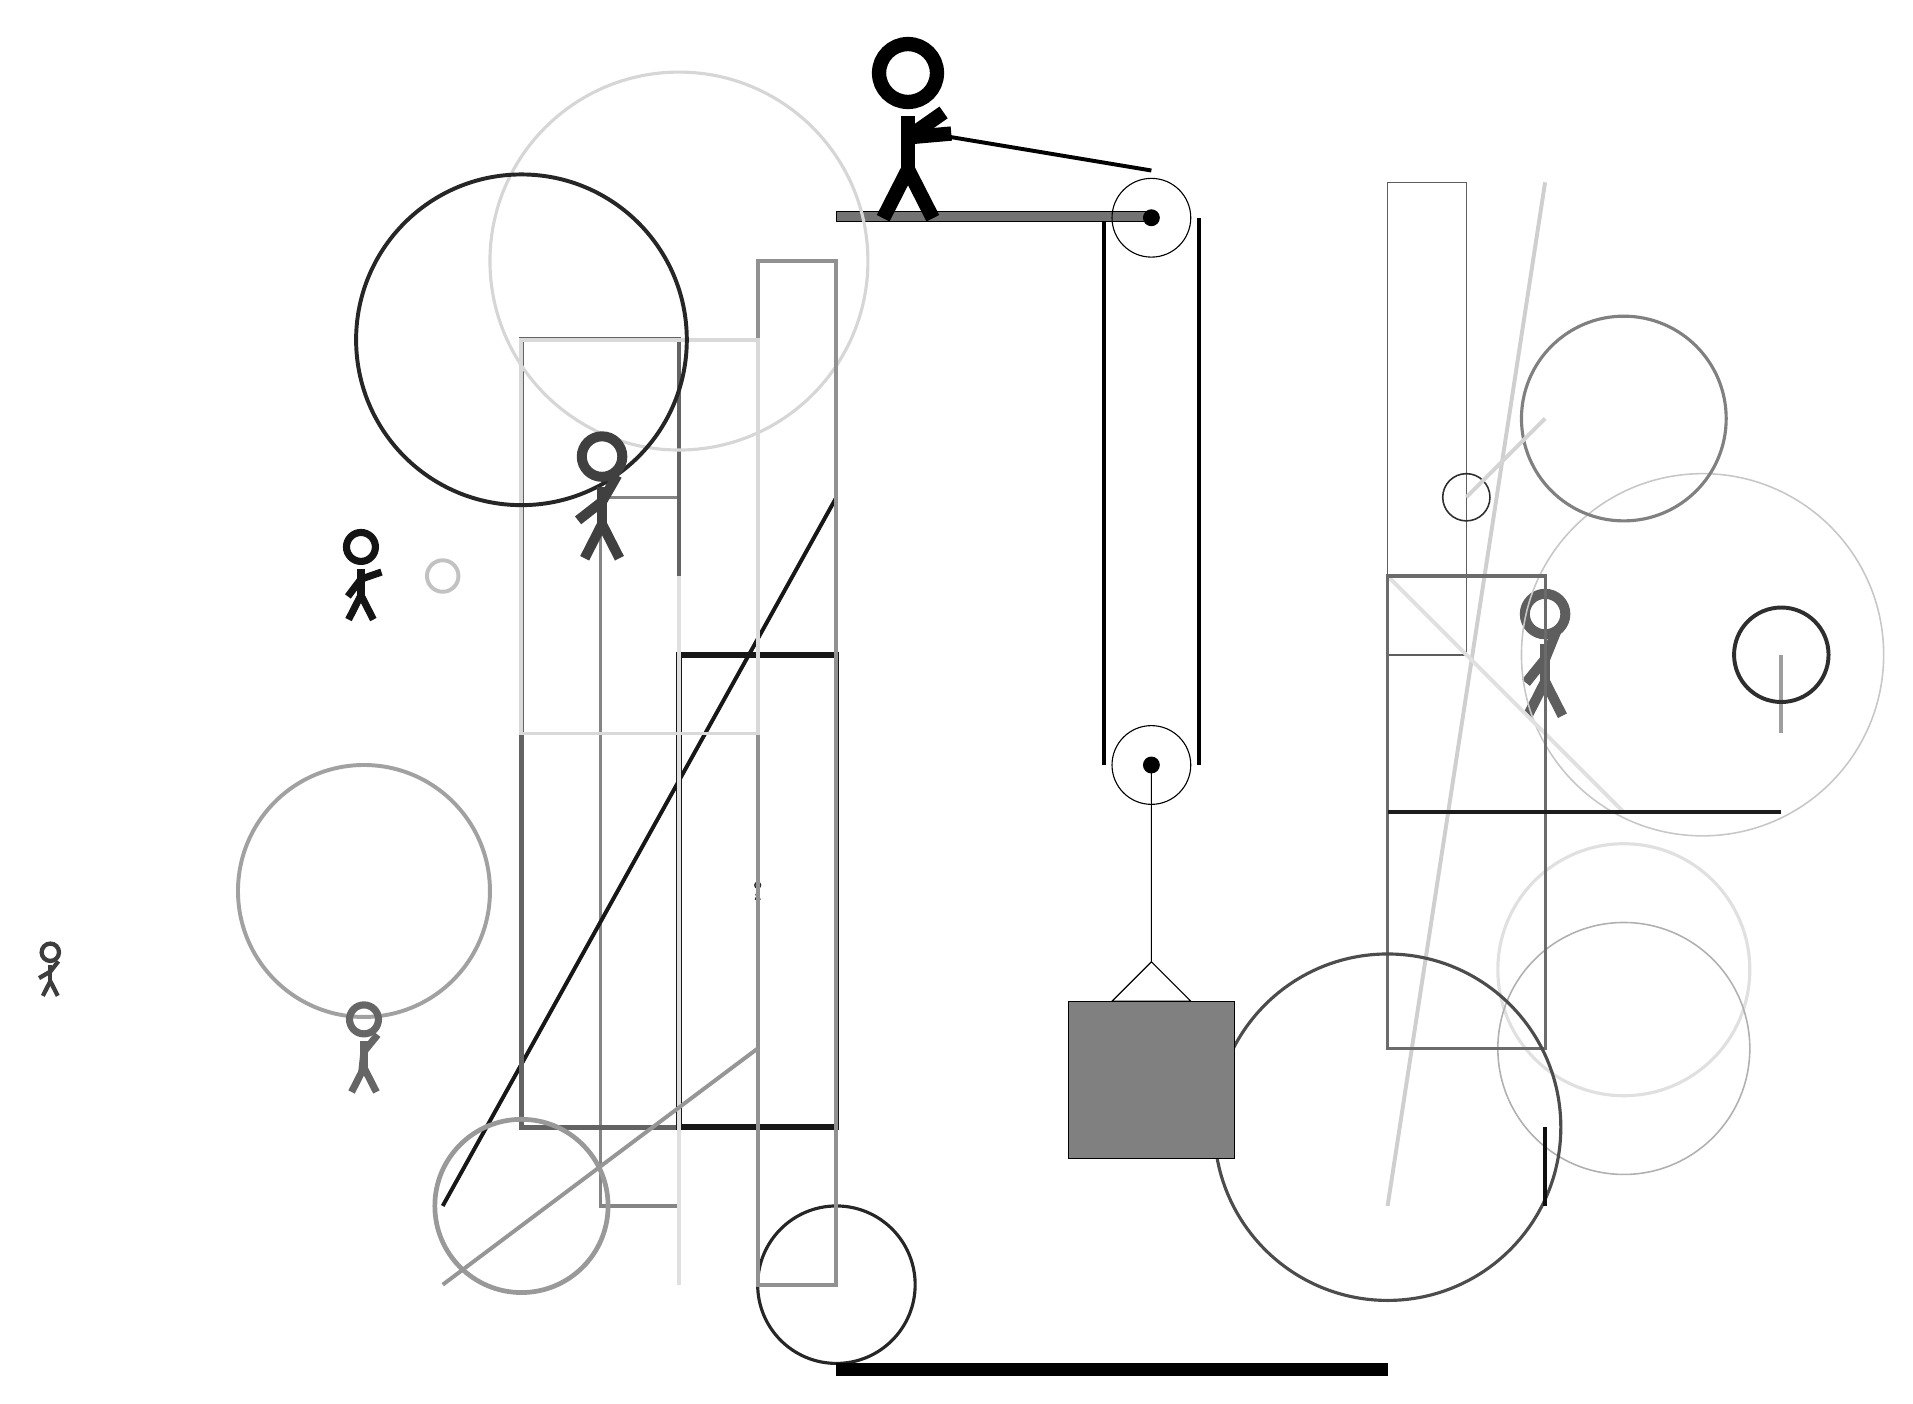
\begin{tikzpicture}
			%%%%% START %%%%%
			
			\draw[fill=black!55] (-2, 11.5) rectangle (2, 11.625);
			
			\draw (2, 4.6) circle (0.5);
			\draw[fill=black] (2, 4.6) circle (0.1);
			
			\draw (2, 11.55) circle (0.5);
			\draw[fill=black] (2, 11.55) circle (0.1);
			
			\draw[line width=0.4mm, color=black!48] (-4, -1) rectangle (-5, 8);
			
			\draw[line width=0.5mm, color=black!91](-2, 8) -- (-7, -1);
			\draw[line width=0.6mm, color=black!61] (-4, 10) rectangle (-6, 0);
			\draw[line width=0.5mm, color=black!19](5, -1) -- (7, 12);
			
			\node[line width=0.6mm, color=black!84] at (-3, 3) {\Strichmaxerl[1][63][76]};
			\draw [line width=0.4mm, color=black!12](8, 2) circle (1.6);
			
			\draw[line width=0.5mm, color=black!38](10, 6) -- (10, 5);
			\node[line width=0.2mm, color=black!63] at (7, 6) {\Strichmaxerl[7][51][68]};
			\draw[line width=0.2mm, color=black!63] (5, 6) rectangle (6, 12);
			\node[line width=0.7mm, color=black!92] at (-8, 7) {\Strichmaxerl[5][53][19]};
			
			\draw [line width=0.2mm, color=black!22](9, 6) circle (2.3);
			\draw [line width=0.4mm, color=black!16](-4, 11) circle (2.4);
			\draw [line width=0.4mm, color=black!85](-2, -2) circle (1.0);
			\draw[line width=0.5mm, color=black!12](8, 4) -- (5, 7);
			\draw [line width=0.2mm, color=black!31](8, 1) circle (1.6);
			\draw [line width=0.5mm, color=black!37](-8, 3) circle (1.6);
			\node[line width=0.2mm, color=black!60] at (-8, 1) {\Strichmaxerl[5][84][51]};
			\draw [line width=0.6mm, color=black!40](-6, -1) circle (1.1);
			\draw[line width=0.7mm, color=black!91] (-4, 0) rectangle (-2, 6);
			\draw[line width=0.4mm, color=black!58] (5, 7) rectangle (7, 1);
			\draw [line width=0.5mm, color=black!24](-7, 7) circle (0.2);
			
			\draw[line width=0.5mm, color=black!43] (-2, -2) rectangle (-3, 11);
			\draw[line width=0.5mm, color=black!15] (-3, 5) rectangle (-6, 10);
			\draw [line width=0.2mm, color=black!82](6, 8) circle (0.3);
			\draw [line width=0.5mm, color=black!85](-6, 10) circle (2.1);
			
			\draw [line width=0.4mm, color=black!50](8, 9) circle (1.3);
			\draw [line width=0.4mm, color=black!70](5, 0) circle (2.2);
			\draw [line width=0.7mm, color=black!53](10, 1) circle (0.0);
			\draw[line width=0.5mm, color=black!89](10, 4) -- (5, 4);
			
			\draw[line width=0.5mm, color=black!17](6, 8) -- (7, 9);
			\draw[line width=0.5mm, color=black!12](-4, 7) -- (-4, -2);
			
			\node[line width=0.5mm, color=black!75] at (-5, 8) {\Strichmaxerl[7][38][60]};
			\node[line width=0.5mm, color=black!76] at (-12, 2) {\Strichmaxerl[3][30][52]};
			
			\draw[line width=0.5mm, color=black!94](7, -1) -- (7, 0);
			
			\draw [line width=0.5mm, color=black!82](10, 6) circle (0.6);
			\draw[line width=0.5mm, color=black!41](-3, 1) -- (-7, -2);
			
			
			\draw (2, 4.6) -- (2, 2.1) -- (1.5, 1.6) -- (2.5, 1.6) -- (2, 2.1);
			\draw[fill=black!50] (0.95, 1.6) rectangle (3.05, -0.4);
			
			\draw[line width=0.5mm] (1.4, 11.5) -- (1.4, 4.6);
			\centerarc[line width=0.5mm](2, 4.6)(180:360:0.6);
			\draw[line width=0.5mm](2.6, 4.6) -- (2.6, 11.55);
			\centerarc[line width=0.5mm](2, 11.55)(0:90:0.6);
			\draw[line width=0.5mm](2, 12.15) -- (-1, 12.65);
			
			\node at (-1, 12.65) {\Strichmaxerl[10][-175][35]};
			
			\draw[fill=black] (-2, -3) rectangle (5, -3.15);
			
			%%%%% END %%%%%
		\end{tikzpicture}
	\end{figure}	
\end{document}